\documentclass{article} % For LaTeX2e
\usepackage{iclr2017_conference,times}
\usepackage{amsmath, amsthm}
\usepackage[subscriptcorrection,mtpcal,amsbb]{mtpro2}
\usepackage{hyperref}
\usepackage{url}
\usepackage{enumitem}
\setlist{leftmargin=15pt}
\usepackage{inconsolata}
\usepackage{textcomp}
\usepackage{lastpage}
\cfoot{\thepage\ of \pageref{LastPage}}
\usepackage{makecell}
\usepackage{physics}
\usepackage{tikz}
\usetikzlibrary{arrows,positioning,automata}
\usetikzlibrary{shapes.geometric}
\usepackage{float}
\usepackage{subcaption}
\usepackage{array}
\newcolumntype{L}[1]{>{\raggedright\let\newline\\\arraybackslash\hspace{0pt}}m{#1}}
\newcolumntype{C}[1]{>{\centering\let\newline\\\arraybackslash\hspace{0pt}}m{#1}}
\newcolumntype{R}[1]{>{\raggedleft\let\newline\\\arraybackslash\hspace{0pt}}m{#1}}
\usepackage{colortbl}


\lhead{\textsc{IFT6135 Representation Learning}}
\rhead{S. Laferri\`ere \& J. Litalien}

\title{Assignment 2 --- Practical Part \\
Convolutional Neural Networks}

\author{Samuel Laferri\`ere\thanks{Student ID 20XXXXXX}\ \, \& Joey Litalien\thanks{Student ID 20122880} \\
IFT6135 Representation Learning, Winter 2018\\
Universit\'e de Montr\'eal\\
Prof. Aaron Courville \\
\texttt{$\{$samuel.laferriere.cyr,joey.litalien$\}$@umontreal.ca}}

\def\*#1{\mathbf{#1}}
\DeclareMathOperator{\ex}{\mathbb{E}}
\DeclareMathOperator{\Var}{Var}

\begin{document}
\maketitle
\thispagestyle{empty}

\section{Regularization}
\begin{enumerate}[label=(\alph*)]
\item \textit{Early stopping and weight decay.} We plot the $L^2$-norm of all parameters $\*w$ at each minibatch update for 100 epochs. To adapt the loss for minibatch SGD, we rescaled the regularization coefficient as $\lambda \gets \lambda b / |\*X|$, where $b$ is the batch size and $\*X$ is the entire training set. We also plot the average loss on the training set for both schemes.
\begin{figure}[ht]
\centering
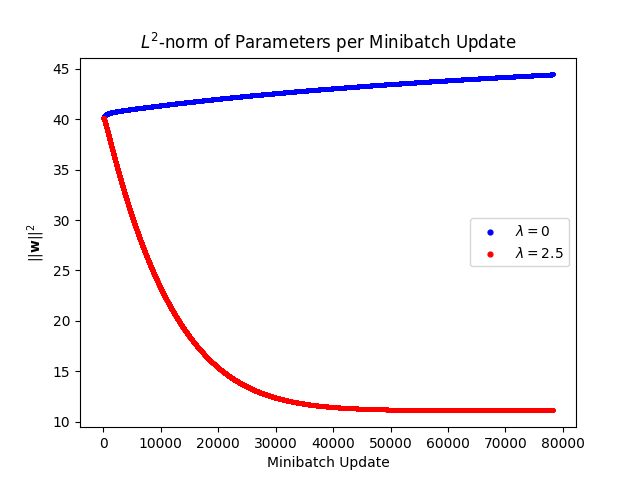
\includegraphics[scale=0.42]{plots/1a_norm.png}
\vspace{5mm}

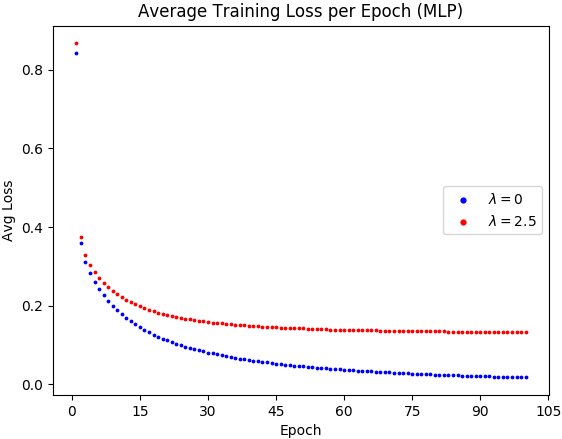
\includegraphics[scale=0.42]{plots/1a_loss.png}
\end{figure}

 
 \newpage
\item \textit{Dropout.}
\item \textit{Convolutional networks.}
We plot the error at the end of each epoch for the model.
\begin{figure}[ht]
\centering
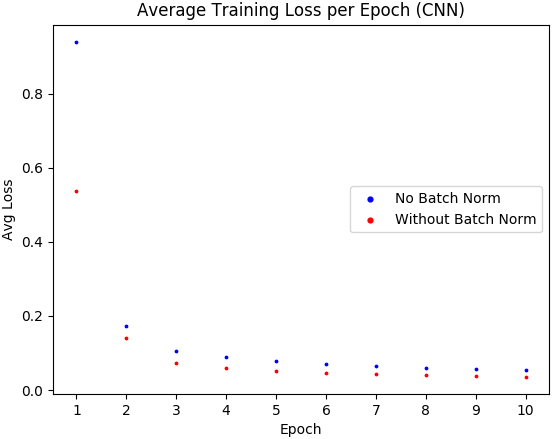
\includegraphics[scale=0.42]{plots/1c_loss.png}
\end{figure}

\end{enumerate}

\section{Dogs vs. Cats Classification}
We have resized the images to $3 \times 64 \times 64$ pixels using the Python script provided and separated the dataset into training/valid/test sets as follows. The index ranges apply to both dogs and cats, making each subsets' class distributions equal.
\begin{table}[ht]
\centering
\begin{tabular}{r C{6.3cm}  C{2.1cm} C{2.1cm} }
Index range & \footnotesize{$[0, 7\,499$]} & \footnotesize{$[7\,500, 9\,999]$} & \footnotesize{$[10\,000,12\,499]$} \\
\cline{2-4}
Dataset & \multicolumn{1}{|c}{\cellcolor{blue!30}\textsc{Train}} & \multicolumn{1}{|c|}{\cellcolor{red!30}\textsc{Valid}} & \multicolumn{1}{c|}
{\cellcolor{yellow!30}\textsc{Test}} \\
\cline{2-4}
Size & \footnotesize{15\,000} & \footnotesize{5\,000} & \footnotesize{5\,000} \\
\end{tabular}
\caption{Splitting the Dogs vs. Cats dataset.}
\end{table}

\begin{enumerate}[label=(\alph*)]
\item \textit{Architecture.}
\item \textit{Performance on test set.}
\item \textit{Visualization and possible improvements.}
\end{enumerate}

















\end{document}